\chapter{Selección del Tipo de Motor}

Los motores lineales son máquinas eléctricas que producen movimiento lineal, en contraste con los motores eléctricos convencionales, que producen movimiento rotatorio. A lo largo de la historia, desde su origen alrededor de 1970 \cite{laithwaite1970}, se han propuesto como alternativas para la producción de movimiento lineal en diferentes ámbitos, así como diferentes configuraciones análogas a las que se encuentran para los motores rotatorios.

De acuerdo a los objetivos del proyecto, se procedió a realizar un estudio de diferentes configuraciones de motores lineales, teniendo en cuenta sus características electromagnéticas y mecánicas, y las aplicaciones encontradas en la industria, con el fin de seleccionar una configuración apropiada para cumplir los requisitos del proyecto. Los resultados fundamentales de este estudio se resumen a continuación.

\section{Motores lineales de inducción}
% Introducción teórica
Los motores lineales de inducción (MLIs) funcionan bajo el principio de los motores de inducción convencionales, en los cuales se tiene un estator con devanado trifásico y un secundario consistente en una lámina de metal conductor en la cual se generan corrientes inducidas por el \textbf{primario}, en el que se encuentra el devanado trifásico, como se muestra en la figura \ref{lim1}. El hierro se añade con el fin de disminuir la reluctancia total del circuito magnético \cite{guru2001}.

\begin{figure}[hbtp]
\centering
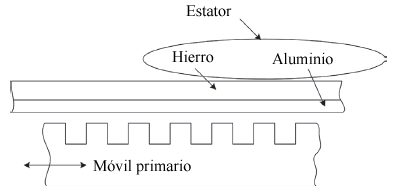
\includegraphics[scale=0.5]{../img/lim1.png}
\caption{Motor lineal de inducción. Tomado de \cite{boldea2013}.}
\label{lim1}
\end{figure}

A partir del análisis de la fuerza magnetomotriz existente en el devanado \cite{boldea2013}, se obtiene que la velocidad del campo magnético viajero es

\begin{equation}
v_s = 2\tau f
\end{equation}

Donde $\tau$ es el paso polar y $f$ es la frecuencia de la fuente de voltaje. El campo viajero induce corrientes en el secundario, y la interacción entre el campo y las corrientes inducidas produce el movimiento lineal. Una vez la velocidad relativa entre el primario y el secundario es cero, las corrientes inducidas y la fuerza ejercida desaparecen, reduciendo nuevamente la velocidad. Este proceso, también presente en los motores de inducción convencionales, se repite hasta que el móvil alcanza una velocidad que nunca será igual a la velocidad de sincronismo $v_s$. Por esta razón, los motores de inducción también reciben el nombre de motores \textbf{asíncronos}.

\subsection{Clasificación según el tipo de primario}
% Características específicas y relevantes de los motores lineales
% - Características, dinámica y eficiencia
Un motor lineal puede ser de \textbf{primario corto} cuando el devanado trifásico se encuentra en el móvil y las láminas conductoras se encuentran en la vía; o de tipo \textbf{primario largo} cuando el devanado trifásico se encuentra extendido a lo largo de la vía y las láminas conductivas constituyen parte del móvil \cite{laithwaite1970}. En el caso del motor de primario corto, es necesario alimentar el móvil con la fuente de alimentación necesaria, lo que hace necesaria la inclusión de baterías junto con convertidores de potencia que aumentan el peso del móvil. Por otro lado, en un motor de primario largo en el que el móvil no requiere de una fuente de alimentación, es necesaria la construcción de un devanado trifásico a lo largo de toda la vía, incrementando los costos debido a la cantidad de cobre necesaria y el material ferromagnético usado en las láminas en las que se incrusta el devanado. Por esta razón, los motores de primario corto son usados en aplicaciones de baja velocidad (hasta alrededor de 100 km/h), mientras que los de primario largo se utilizan en altas velocidades, en las que la alimentación de energía del móvil sería impráctica \cite{leekimlee2006}.

\subsection{Efecto de extremos}
% - Efecto de extremos
En los motores rotatorios convencionales, el rotor consiste en un cilindro cuya superficie es continua. Este, sin embargo, no es el caso en los motores lineales. En los MLIs se producen corrientes de inducción en el secundario adicionales debidas a su entrada y salida del campo magnético viajero establecido por el primario, como se muestra en la Fig. \ref{eelim}. Este efecto se conoce como \textbf{efecto de extremos} o \textbf{efecto dinámico longitudinal} \cite{boldea2013}, que reduce la eficiencia de los MLIs y sy factor de potencia \cite{bazghaleh2010,selcuk2008}. 

\begin{figure}[hbtp]
\centering
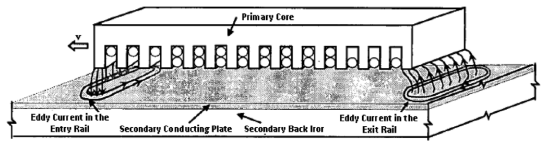
\includegraphics[scale=0.6]{../img/eelim.PNG}
\caption{Efecto de extremos en un MLI. Tomado de \cite{bazghaleh2010}.}
\label{eelim}
\end{figure}

De acuerdo a \cite{boldea2013}, el efecto de extremos se puede ignorar en el caso en el que el factor de \textit{goodness} $G$ (definido en \cite{laithwaite1965}) cumple con la relación
\begin{equation}
\frac{\tau}{\pi}G < \frac{L_p}{10}
\label{endeffectcond}
\end{equation}
donde $\tau$ es el paso polar del motor y $L_p$ es la inductancia del primario. Así, para altas velocidades, donde la frecuencia crece, $G$ aumenta, indicando que el efecto de extremos es menos restrictivo en máquinas de baja velocidad, a pesar de tener un factor $G$ menor.

Para los casos en que este efecto no puede ser despreciado, se han propuesto soluciones en el diseño y el control de los MLIs que permiten reducirlo, como se muestra en \cite{bazghaleh2010,kuznetsov2008,guo2012,zhang2012}.

\subsection{Efecto pelicular}
% - Efecto skin
El efecto pelicular suele caracterizarse a partir de la distancia de la superficie a la cual la densidad de corriente se ha reducido en un factor de $e$ ($\approx$ 2.781) \cite{boldea2010}, conocida como la profundidad de penetración $\delta$. En los motores lineales, se encuentra que este efecto reduce la densidad de flujo magnético en el entrehierro. Este efecto puede mitigarse al utilizar un estator laminado y aislado, lo que se traduce en una reducción de $\sigma$, obteniéndose un incremento en la densidad de flujo magnético pico de aproximadamente el doble \cite{boldea2013}.

La consideración del efecto pelicular en el diseño de MLIs ha sido amplia en los trabajos realizados en el área, debido a que los modelos simplificados que no tienen en cuenta este efecto llegan a resultados que difieren del comportamiento obtenido en un motor real \cite{gieras1986}. Se han propuesto diferentes modelos de circuito equivalente que tienen en cuenta la dinámica del motor así como los efectos de extremos y pelicular, que mejoran el modelado del motor con el fin de estudiar aspectos como la eficiencia, el factor de potencia y el empuje, y proporcionar un modelo que sea útil en el diseño y control de los MLIs \cite{weixu2007,weixu2008,weixu2009,dong2014}.

\section{Motores lineales sincrónicos con sistema de excitación}
En los motores lineales síncronos con sistema de excitación (MLS), se reemplaza la lámina conductora de los MLIs por una estructura con una fuente de campo magnético (utilizando imanes permanentes, electroimanes o superconductores) de manera que los polos se alinean con el campo magnético viajero producido por el devanado trifásico, como se muestra en la Fig. \ref{lsm2}.

\begin{figure}[hbtp]
\centering
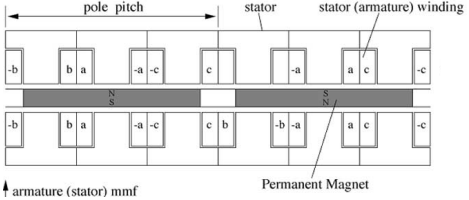
\includegraphics[scale=0.6]{../img/lsm2.PNG}
\caption{MLS de imanes permanentes con doble armadura. Tomado de \cite{stumberger2004}.}
\label{lsm2}
\end{figure}

La fuente de excitación para crear el campo magnético puede variar de acuerdo a la aplicación. Para distancias cortas (alrededor de 10 m, como en aplicaciones industriales), se pueden utilizar imanes permanentes (ver Fig. \ref{lsm1}), mientras que para distancias más largas, donde el costo de una larga serie de imanes sería prohibitivo (como en sistemas de transporte), se utiliza excitación electromagnética \cite{gieras2000}. Los MLS son más utilizados en aplicaciones de alta velocidad (mayor a 100 km/h). Debido a que son compatibles con sistemas de suspensión electrodinámica, son comúnmente usados en sistemas de transporte urbano para la propulsión de trenes de levitación magnética \cite{boldea2013,leekimlee2006}.  A continuación se describen los sistemas de excitación utilizados en la industria.

\begin{figure}[hbtp]
\centering
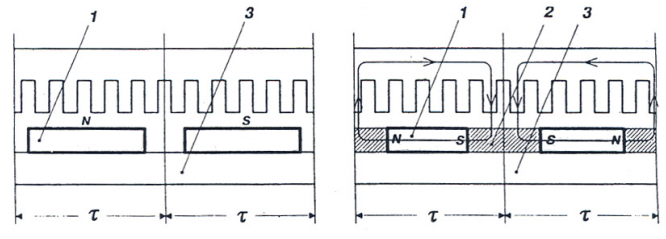
\includegraphics[scale=0.7]{../img/lsm1.PNG}
\caption{Dos tipos de MLS: de imanes superficiales (izquierda) y enterrados (derecha). 1: imanes permanentes. 2: polos de acero. 3: yugo. Tomado de \cite{gieras2000}.}
\label{lsm1}
\end{figure}

\subsection{MLS de imanes permanentes}
Como ya se describió anteriormente, los MLS de imanes permanentes utilizan estos elementos como sistema de excitación. La configuración mostrada en la Fig. \ref{lsm1} utiliza un yugo ferromagnético de alta permeabilidad para proveer un camino de baja reluctancia para la densidad de flujo magnético.

La configuración de imanes conocida como el  \textbf{arreglo de Halbach} \cite{mallison1973} es también utilizada en los sistemas de excitación de los MLS. La distribución del campo que genera este arreglo se muestra en la Fig. \ref{halbachsimulation}. Debido a las características del campo magnético generado, este arreglo ha sido propuesto en el uso de motores sincrónicos rotatorios y lineales, debido a que evitan la necesidad de utilizar material ferromagnético, reduciendo así las pérdidas en el núcleo (por histéresis y corrientes parásitas) y además, en el caso de los motores lineales, proveen de un aislamiento magnético que puede ser importante en los trenes de transporte, donde los fuertes campos magnéticos pueden representar un riesgo de salud para los pasajeros \cite{trumper1993,trumper1994}.

\begin{figure}[h]
\centering
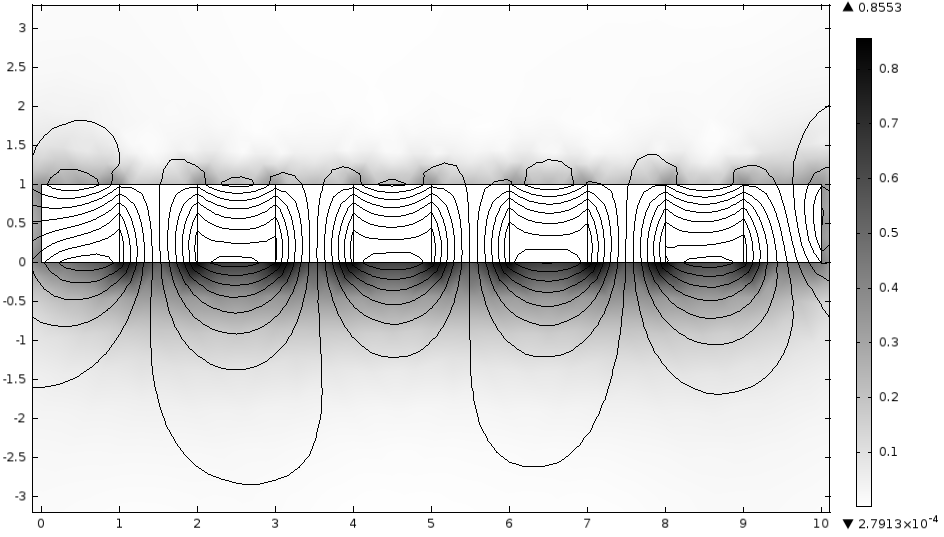
\includegraphics[scale=0.4]{../img/halbachsimulation.PNG}
\caption{Simulación del arreglo de Halbach. Superficie: densidad de flujo magnético (T). Líneas de contorno: Vector potencial magnético.}
\label{halbachsimulation}
\end{figure}


El uso de los imanes permanentes en el sistema de excitación, junto con una armadura con material ferromagnético, produce un efecto no deseado conocido como la \textbf{fuerza de detención}, debida a la atracción entre los imanes y el material ferromagnético. Esta fuerza produce rizado en el movimiento, vibración y ruido en estos motores. Esta situación puede ser mejorada por medio de un posicionamiento inclinado de los imanes \cite{gieras2000}, o a partir de un efecto combinado entre la inclinación de los imanes y un cambio en su geometría, como se muestra en \cite{seokjang2002,tavana2010}.

Aunque el uso de imanes permanentes evita la construcción de un sistema de excitación activo (como el descrito en la siguiente sección), estos están construidos con materiales costosos, como los imanes de NdFeB (una aleación de neodimio, hierro y boro). El uso de este tipo de imanes puede incrementar el costo de un sistema de excitación \cite{gieras2000}.
% Los imanes son caros!

\subsection{MLS de excitación electromagnética}
Los MLS con este tipo de excitación generan el campo magnético con electroimanes, que consisten en bobinas alimentadas con corriente DC, montadas alrededor de un núcleo ferromagnético, extendidas longitudinalmente y con polaridad alternante. Una sección de este sistema se muestra en la Fig. \ref{lsm_eme}.

\begin{figure}[hbtp]
\centering
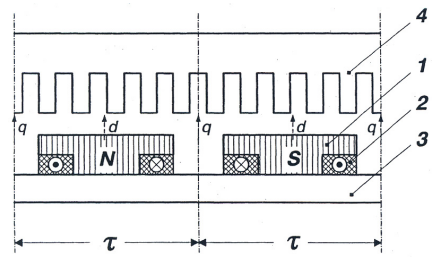
\includegraphics[scale=0.6]{../img/lsm_eme.PNG}
\caption{Sistema de excitación electromagnética en un MLS. 1: núcleo ferromagnético. 2: bobina de campo. 3: yugo. 4: armadura. Tomado de \cite{gieras2000}.}
\label{lsm_eme}
\end{figure}

Este tipo de excitación se convierte en una alternativa para los sistemas de excitación con imanes permanentes, por lo que son usados en sistemas de propulsión con motores lineales donde el costo de los imanes permanentes es prohibitivo, como el  Transrapid de Alemania \cite{leekimlee2006}.

No obstante, el uso de electroimanes implica la inclusión de una fuente de alimentación y circuitos electrónicos de potencia para el manejo y control del sistema de excitación, así como un método adecuado para la transmisión de energía \cite{shibata1992,andriollo1997,minchen2004}.

\subsection{MLS de excitación con superconductores}
Este tipo de excitación es utilizado en grandes MLS, donde el sistema de excitación consiste en electroimanes construidos con superconductores, de forma que no es necesario incluir un núcleo ferromagnético, debido a que producen una densidad de flujo mucho mayor a la del flujo de saturación de las mejores aleaciones ($\approx$ 2.4 T) \cite{gieras2000}. Es encontrado en los trenes de levitación más rápidos que se han construido, como el MLX de Japón, con una velocidad de entre 580 km/h y 600 km/h \cite{leekimlee2006}. Debido a que la construcción de este tipo de motores es práctica para potencias de cientos de kW, los MLS de excitación con superconductores no serán tenidos en cuenta para este proyecto.

\section{Motores lineales de reluctancia variable}
Los motores lineales de reluctancia variable, o simplemente de reluctancia (MLR) funcionan debido a la magnetización de un núcleo ferromagnético anisotrópico \cite{chapman2003}. Esto permite obtener un motor que se mueve a velocidad sincrónica, sin necesidad de un sistema de excitación como imanes o electroimanes, como es el caso de los MLS. Los MLR son utilizados en aplicaciones de transporte de media y alta velocidad  y aplicaciones industriales de coto recorrido \cite{boldea2013}. Debido a que consisten en un sistema dinámico variante en el tiempo (dado que la reluctancia del motor varía con la posición), son motores para los cuales es necesario diseñar estrategias de control más elaboradas (en comparación con las propuestas en el control clásico), como el lazo doble de realimentación de corriente y velocidad, con una tabla de consulta (\textit{lookup table}) para la linealización de la fuerza, propuesto en \cite{waichuen2003}, o el adaptivo de modo deslizante propuesto en \cite{pupadubsin2012} y \cite{habeeb2014}, que resulta robusto frente a variaciones en el modelo dinámico, perturbaciones y las no linealidades presentes en este tipo de motor. 

En la Fig. \ref{lrm1} se observa este tipo de motor. El núcleo ferromagnético tiene una geometría compuesta por ranuras y polos salientes que conforman una reluctancia variable a lo largo del movimiento. En esta figura, los ejes \textit{d} y \textit{q} corresponden a \textit{direct} y \textit{quadrature}, o directo y cuadratura.

\begin{figure}[hbtp]
\centering
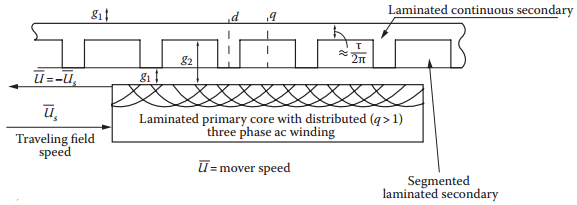
\includegraphics[scale=0.7]{../img/lrm1.PNG}
\caption{Motor lineal de reluctancia. Tomado de \cite{boldea2013}.}
\label{lrm1}
\end{figure}

Los MLR funcionan con un buen desempeño, en cuanto al empuje mínimo requerido, cuando la razón entre la inductancia a lo largo del eje d $L_d$ y a lo largo del eje q $L_q$ es tal que $L_d/L_q \geq 3$ \cite{gieras2000}.

Como puede observarse, los MLR requieren de una estructura especial construida con material ferromagnético para su funcionamiento, que garantice la variación de la reluctancia en el sentido del movimiento. Esto puede incrementar los costos con respecto a motores como los MLI, donde se utiliza una lámina de material conductor sin ranuras. Así como en el caso de los motores rotatorios de reluctancia, debido a su naturaleza, los MLR sufren de rizado en el empuje, produciendo vibraciones y ruido durante el movimiento. Estos efectos pueden reducirse al utilizar barreras de flujo en el secundario como las mostradas en la Fig. \ref{lrmfluxbarriers}. Sin embargo, estas configuraciones requieren de una construcción más especializada y material aislante adicional como la resina epoxy \cite{gieras2000}, incrementando los costos en este tipo de secundarios.

\begin{figure}[hbtp]
\centering
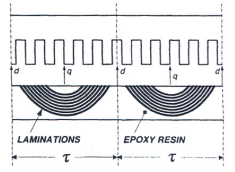
\includegraphics[scale=1]{../img/lrmfluxbarriers.PNG}
\caption{Barreras de flujo para la disminución del rizado en el torque. Tomado de \cite{gieras2000}.}
\label{lrmfluxbarriers}
\end{figure}

Debido a la diferencia de la inductancia en los ejes d y q en los MLR, se generan armónicos de orden superior que incrementan las pérdidas en el material ferromagnético, disminuyendo la eficiencia de este tipo de motores \cite{boldea2013}. Por esta razón, es necesario utilizar un secundario laminado que disminuya este tipo de pérdidas.

Un caso específico de los MLR son los motores lineales de reluctancia conmutada, con los cuales es necesaria la inclusión de sensores de posición que permiten conocer la posición del secundario con respecto al primario, con el fin de aprovechar el empuje efectuado por cada fase \cite{boldea2013}. Una vez conocida la posición del secundario, las fases se conmutan de forma que se produzca el movimiento en la dirección deseada, razón por la cual estos motores recibe su nombre.

\section{Características comunes en los motores lineales}
 
Entre las características mencionadas para cada tipo de motor lineal, existe una en común y es debida a la discontinuidad en el circuito magnético en motores lineales donde el elemento más largo corresponde a la estructura con el devanado trifásico, donde la sección corta del motor actúa como una carga móvil que produce un desbalance en las tres fases, causando corrientes conocidas como \textbf{corrientes de circulación} \cite{jang2010}.

Por otro lado, es importante tener en cuenta que los motores sincrónicos (con sistema de excitación o de reluctancia) tienen torque de arranque cero. Un método para sortear este problema consiste en agregar una lámina amortiguadora de material conductor (análoga a los devanados amortiguadores utilizados en los motores rotatorios sincrónicos \cite{chapman2003}) que ayuda a reducir las oscilaciones en el movimiento del motor \cite{gieras2000}. Otros métodos contemplan la utilización de un variador de frecuencia electrónico, tal como los usados en los motores rotatorios \cite{chapman2003}.

Tanto los MLI como los MLS han sido utilizados en sistemas de transporte. Sin embargo, de acuerdo a los sistemas implementados actualmente o propuestos en diversas partes del planeta, puede observarse una diferenciación de acuerdo a su velocidad, como se muestra en el cuadro. Es claro que para velocidades superiores a los 100 km/h, es preferido el uso de los MLS, debido a los inconvenientes anteriormente descritos para los MLI, que se vuelven suficientemente problemáticos a estas velocidades para no ser considerados.

\begin{table}[hbtp]
\caption{Tipos de motores utilizados en la propulsión de trenes de transporte \cite{leekimlee2006}.}
\centering
\begin{tabular}{c c c}
\textbf{Sistema} & \textbf{Velocidad (km/h)} & \textbf{Tipo de motor}\\
\hline \\
HSST (Japón) & 100 & MLI \\
Transrapid (Alemania) & 500 & MLS \\
MLX (Japón) & 581 & MLS \\
UTM (Corea) & 110 & MLI \\
Swissmetro (Suiza) & 500 & MLS \\
Inductrack (EEUU) & 500 & MLS \\
\end{tabular}
\label{lmtrains}
\end{table}

A partir de los resultados citados anteriormente y además, de \cite{hassanpour2008,vaezzadeh2006,shin2015,dongyeuplee2005,abdelaziz2008,perreault2009}, se puede obtener un conjunto de resultados comparativos en cuanto a la eficiencia y el factor de potencia para los tres tipos de motores lineales mencionados. En total, se tuvieron en cuenta 38 motores, de los cuales 28 especificaban el factor de potencia obtenido. En la Fig. \ref{fig:effs} se visualizan los resultados obtenidos. En la Fig. \ref{fig:effsdata} se observa la eficiencia obtenida para los motores lineales en casos particulares. En esta gráfica puede observarse que cada tipo de motor puede agruparse en un rango de eficiencia, como se puede observar en la Fig. \ref{fig:effsbands}, donde cada rectángulo indica los valores mínimos y máximos de eficiencia obtenidos para cada tipo de motor.

\begin{figure}[t]
    \centering
    \begin{subfigure}[b]{0.49\textwidth}
        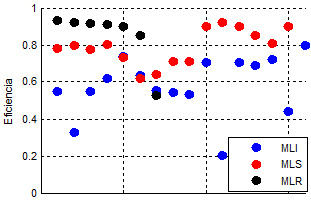
\includegraphics[width=\textwidth]{../img/effsdata.PNG}
        \caption{Resultados para casos particulares.}
        \label{fig:effsdata}
    \end{subfigure}
    ~ %add desired spacing between images, e. g. ~, \quad, \qquad, \hfill etc. 
      %(or a blank line to force the subfigure onto a new line)
    \begin{subfigure}[b]{0.49\textwidth}
        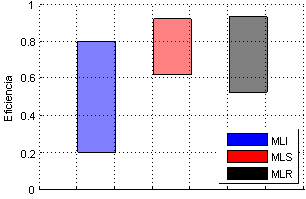
\includegraphics[width=\textwidth]{../img/effsbands.PNG}
        \caption{Rangos de eficiencia para cada tipo.}
        \label{fig:effsbands}
    \end{subfigure}
    \caption{Resultados de eficiencia, obtenidos para diferentes tipos de motores lineales.}\label{fig:effs}
\end{figure}

En la Fig. \ref{fig:pfs} se muestran dos gráficas similares, en este caso para el factor de potencia obtenido en estos trabajos. Los datos obtenidos permiten identificar un rango amplio de valores para el factor de potencia.

\begin{figure}[t]
    \centering
    \begin{subfigure}[b]{0.49\textwidth}
        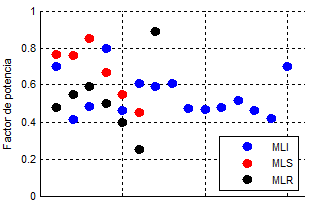
\includegraphics[width=\textwidth]{../img/pfdata.PNG}
        \caption{Resultados para casos particulares.}
        \label{fig:pfdata}
    \end{subfigure}
    ~ %add desired spacing between images, e. g. ~, \quad, \qquad, \hfill etc. 
      %(or a blank line to force the subfigure onto a new line)
    \begin{subfigure}[b]{0.49\textwidth}
        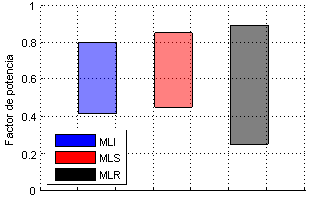
\includegraphics[width=\textwidth]{../img/pfbands.PNG}
        \caption{Rangos del factor de potencia para cada tipo.}
        \label{fig:pfbands}
    \end{subfigure}
    \caption{Resultados del factor de potencia, obtenidos para diferentes tipos de motores lineales.}\label{fig:pfs}
\end{figure}

\begin{table}[hbtp]
\caption{Características para diferentes tipos de motores.}
\centering
\begin{tabular}{c c c c}
& \textbf{MLI} & \textbf{MLS} & \textbf{MLR}\\
\hline
\textbf{Eficiencia} & 0.2-0.8 & 0.6-0.9 & 0.5-0.9 \\
\textbf{Factor de potencia} & 0.4-0.8 & 0.5-0.8 & 0.2-0.9 \\
\textbf{Secundario} & Conductor & Activo & Reluctancia\\
\textbf{Potencia} & Cientos de vatios & Miles de vatios & Cientos de vatios \\
\end{tabular}
\label{motorfeatures}
\end{table}

\section{Selección del tipo de motor}
Los objetivos del proyecto plantean la optimización del diseño de un motor eléctrico lineal de 100 W para una carga de 2 kg, para el cual se diseñará un controlador de velocidad, a partir de lo cual se definieron los requisitos del motor y el diseño de la siguiente forma:

\begin{itemize}
\item Potencia de 100 W para una carga de 2 kg.
\item Eficiente en términos del uso de la energía.
\item Restringido en el uso de materiales costosos.
\end{itemize}
% Hasta acá

Dentro de este contexto, la selección del motor se realizó a partir de los resultados obtenidos durante la revisión del estado del arte. Con respecto a los resultados obtenidos en las secciones anteriores, pueden obtenerse una serie de características relacionadas con las propiedades eléctricas y mecánicas de los diferentes motores, como se resume en la Tabla \ref{motorfeatures}. 

En primera instancia, se observa que con respecto a la potencia, las implementaciones tienden a valores bajos en el caso de los MLI y los MLR, siendo utilizados en aplicaciones industriales o en sistemas de transporte de baja velocidad, en comparación con los MLS utilizados en sistemas de transporte de alta velocidad y propulsión de aeronaves. 

Los MLS y MLR presentan valores de eficiencia más altos que el MLI. Sin embargo, los MLR se destacan como el tipo de motor que produce mayores factores de potencia.

Las diferencias fundamentales en cada motor se encuentran en el secundario, ya que cada tipo posee una configuración especial, que en el caso de los MLS puede incrementar el costo en su construcción.

Los MLR pueden verse como un motor cuya construcción produce ventajas tomadas de los MLI y los MLS: al no depender de corrientes inducidas, produce una mayor eficiencia que los MLI, y al no utilizar elementos externos para la generación de campo magnético, los costos son menores con respecto al MLS.

Tal como fueron definidos los requisitos del motor, no existe la necesidad de valores altos de potencia, y se busca obtener un motor con alta eficiencia y que no utilice materiales. A partir de los criterios mostrados en la Tabla \ref{motorfeatures} y las consideraciones anteriores, se decidió trabajar con los MLR, debido a que son candidatos para cumplir con los requisitos del proyecto. Además, debido a que son motores que no han sido trabajados de forma tan extensiva como los MLS y los MLI, se presenta la oportunidad de producir resultados relacionados con este tipo de motor que aporten a su adopción en la industria.

\bibliographystyle{ieeetr}
\bibliography{../refs}